The goal of real-time scheduling is to guarantee timing correctness; in other words, every task is schedulable if it meets the predefined timing constraints at design time. Being ``schedulable'' depends on whether task deadlines are hard or soft. %(We consider both possibilities in this research.) 
For a hard real-time (HRT) task, its deadline must be met; while for a soft real-time (SRT) task, missing some deadlines can be tolerated. %For example, in an automotive system, autonomous control and emergent collision avoidance  are  HRT tasks; while automatic lane following and traffic sign recognition can be viewed as SRT tasks. 
 SRT constraints can be defined in several ways. We assume a well-studied SRT notion \cite{mills2010stochastic, erickson2012soft, johndissertation, BBBdissertation, devidissertation, leontyevdissertation} that an SRT task is schedulable if its response time can be provably bounded. (Such bounds would be expected to be reasonably small.) In this research, we consider both HRT and SRT possibilities.  

To guarantee timing correctness, we must develop two kinds of algorithms: \textit{real-time scheduling algorithms} and \textit{schedulability tests}. A scheduling algorithm (i.e., scheduler) determines when to execute which task and on which resource. Scheduling algorithms can usually be divided into two major categories: (\textit{i}) partitioned scheduling, and (\textit{ii}) global scheduling. %, and (\textit{iii}) clustered scheduling. 
Under partitioning, tasks are statically partitioned among processors~\cite{andersson2003, baker2007, funk2005, Baruah2006a, chattopadhyay2011, baruah2005a}. %; i.e., each task is bound to execute on a specific processor and will never migrate to another processor \cite{andersson2003, baker2007, funk2005, Baruah2006a, chattopadhyay2011, baruah2005a}. 
Different processors can apply different scheduling algorithms. An example partitioned scheduler is partitioned earliest-deadline-first (EDF), which uses the EDF algorithm as the per-processor scheduler. (Under EDF, jobs with earlier deadlines have higher priority.) In contrast to partitioning, under global scheduling, a single global ready queue is used for storing ready jobs \cite{baruah2008, bertogna2011b, BC, devi2005}. Jobs are allowed to migrate from one processor to another at any time. A global scheduling algorithm example is global EDF (GEDF), under which jobs are EDF-scheduled using a single ready queue. 
 Clustered scheduling is hybrid of partitioned and global scheduling in which tasks are statically assigned to a cluster of processors, among which the task can freely migrate.
 Note that the ARM's big.LITTLE platform we will focus in this research has implemented the general global and clustered scheduling policies~\cite{armscheduler}. Moreover, under another categorization method of scheduling algorithms, we may have either fixed-priority or dynamic-priority schedulers, where a fixed-priority scheduler assigns a fixed priority to each task and all the jobs released by this task inherit the same task priority (e.g., rate-monotonic scheduling which assigns higher priorities to tasks with shorter periods) and a dynamic-priority scheduler assigns every job a different priority (e.g., EDF).
 
  %On multi- and many-core systems, clusters are often aligned to the underlying hardware architecture so as to prevent expensive migrations between remote cores. It has been shown that such migration overhead reductions could enhance the overall performance in embedded systems with stringent SWaP constraints (e.g., an automotive system)~\cite{bastoni2010}.

%It is executed repeatedly at runtime during the lifetime of a real-time system. 
Depending on the scheduling algorithm being used, at design time a corresponding schedulability test verifies whether a task system will be schedulable, provided that the system behaves according to its parameterized specification. Finding an optimal scheduling algorithm that experiences no capacity loss (i.e., 100\% resource utilization) is not always possible. If a non-optimal scheduling algorithm is used, then a schedulable task system may be deemed unschedulable by the corresponding schedulability test due to algorithmic capacity loss.
Our goal of designing energy-efficient scheduling algorithms and schedulability tests is to minimize the overall capacity loss.% (i.e., maximize resource utilization). 

%In practice, finding an optimal scheduling algorithm that can fully allocate all processor capacity to real-time tasks is not always possible.
%; i.e., task systems with total utilization less than $m$ may not be schedulable on $m$ processors. 
%One primary cause of such capacity loss is due to the choice of a scheduling algorithm. If a non-optimal scheduling algorithm is used, then a schedulable task system may be deemed unschedulable due to algorithmic capacity loss. Our goal of designing resource-conscious scheduling and schedulability analysis algorithms is to minimize the capacity loss on all resources (i.e., maximize resource utilization). 

\begin{comment}

\begin{wrapfigure}{r}{0.46\textwidth}
%	\captionsetup{width=0.65\textwidth}  
\vspace{-4mm}
	\begin{center}
          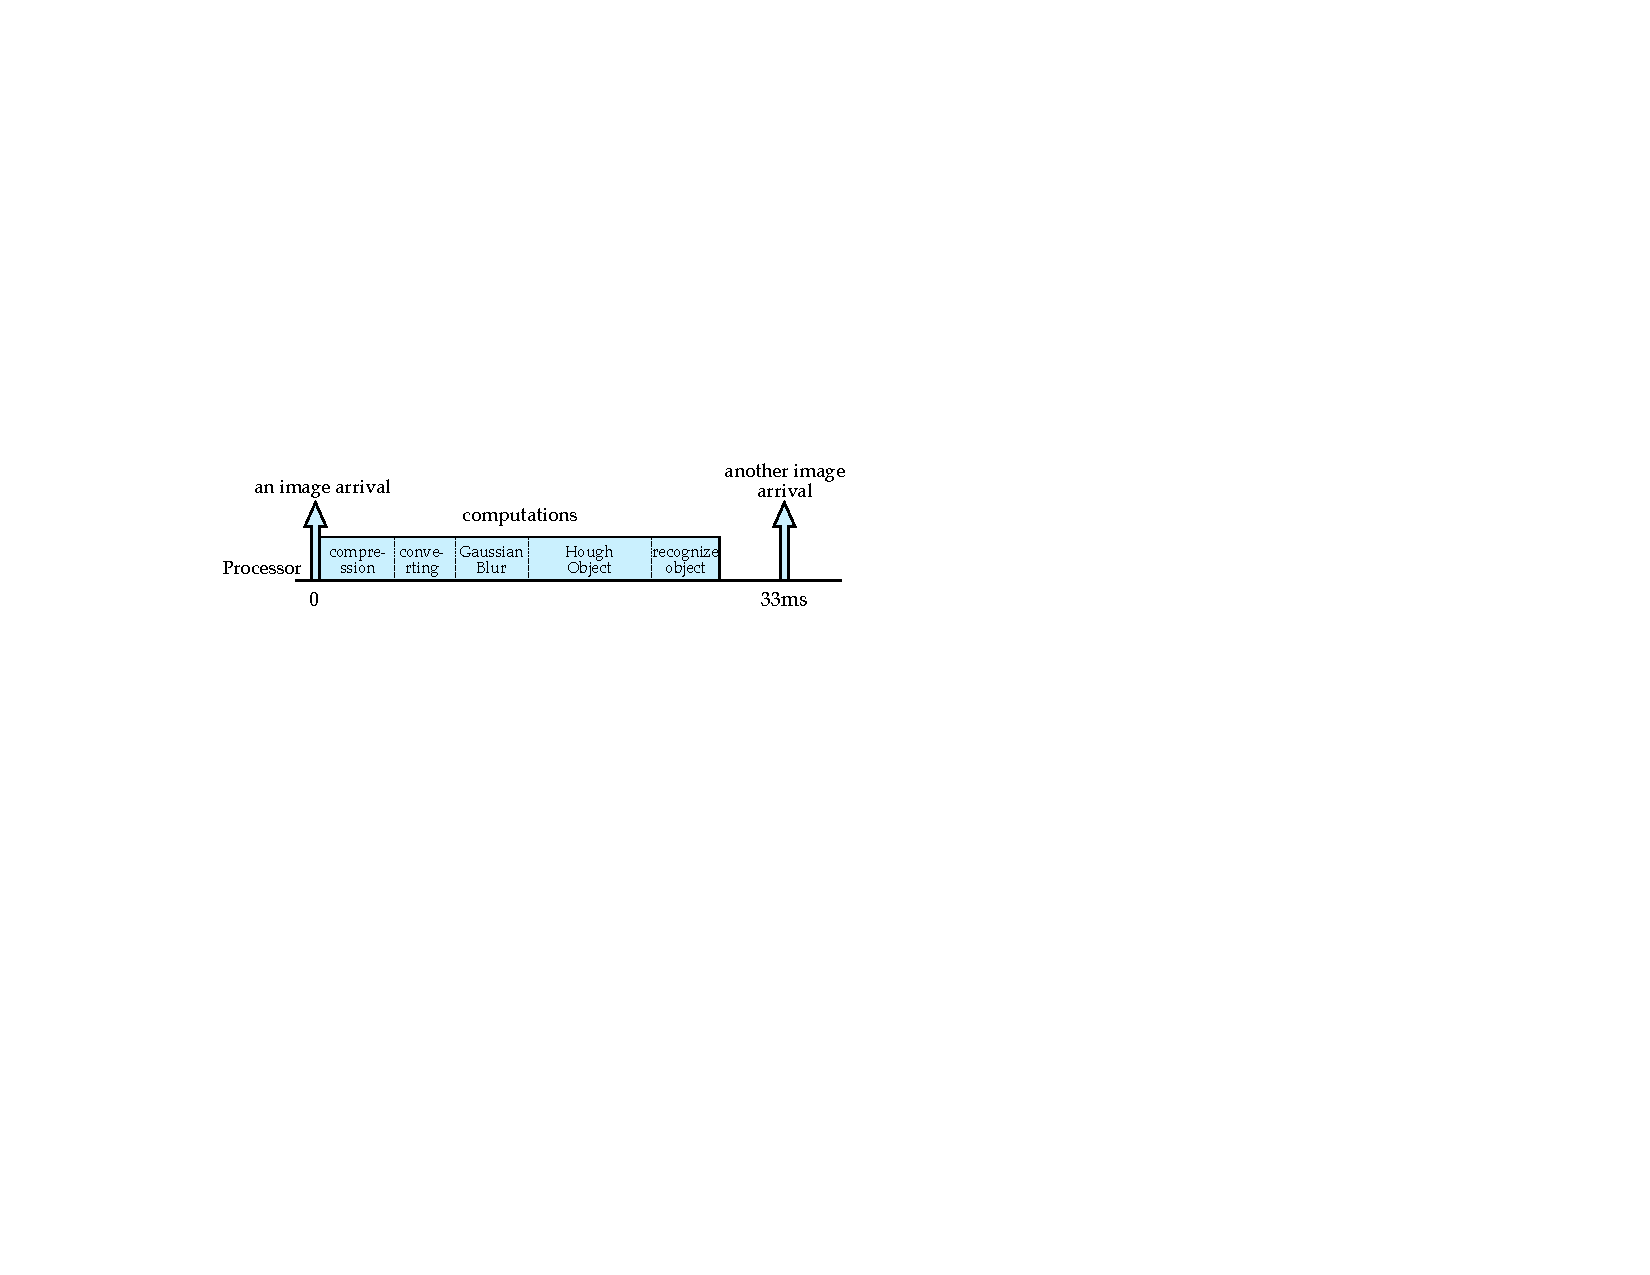
\includegraphics[width=3in]{images/sporadiceg.pdf} 
    \end{center}
    \vspace{-2mm}
\caption{\small The sporadic job releasing pattern of object recognition applications.}
\vspace{-2mm}   
\label{fig:sporadiceg}
\end{wrapfigure} \normalsize
\end{comment}

\paragraph{Workload Models.} Real-time embedded systems commonly perform recurring operations. For example, the object recognition application commonly involved in implementing many autonomous-driving assisted functionality is naturally recurrent. Specifically, the camera sensor captures an image at a certain frequency; each image is compressed and then analyzed using certain object recognition algorithms, and is expected to be completed by the invocation of the next frame; e.g., each invoked job ideally should complete the corresponding workloads within 33\textit{ms} for a 30 frame-per-second camera. %, as illustrated in Figure~\ref{fig:sporadiceg}.  

Generally speaking, a specified real-time system consists of a collection of recurring real-time processes called ``tasks''. %A real-time task is a  program that is repeatedly invoked in response to external events such as device interrupts or expiring timers. When a task is invoked in response to an event, it releases a ``job'' to process the event. 
A widely studied general model of recurrent workloads is the \textit{sporadic task model}~\cite{sporadic}. In this model, the specified system is composed of a collection of recurring\footnote{Although our focus in this document is on the notion of recurrence found in the sporadic model, we intend to consider other such notions in our work.} %Moreover, although recurrent task arrival pattern is dominant in real-time embedded systems, other patterns in practice may exist. As seen in Sec.~\ref{sec:remoteresource}, we will also consider other workload arrival patterns such as non-recurrent and independent jobs that often appear in the emerging mobile embedded systems.} 
sequential tasks, $\tau = \lbrace \tau_1$, ..., $\tau_n \rbrace$. Each such task $\tau_i$ releases a succession of \textit{jobs} $J_{i,1}$, $J_{i,2}$, ... and is defined by specifying a \textit{period} $T_i$, a \textit{relative deadline} $D_i$, and a \textit{worst-case execution time (WCET)} $C_i$. Successive jobs of $\tau_i$ are released at least $T_i$ time units apart, and one that is released at time $t$ has a deadline at time $t+D_i$. Also, each such job executes for at most $C_i$ time units. %Figure.~\ref{fig:modeleg}(b) shows an example sporadic task that models a simple control application.
Each job released by any task has a \textit{response time} that defines the duration from its release to its finish time. A task $\tau_i$'s response time equals the maximum job response time among all of its released jobs. 

%The sporadic task model has received an enormous amount of attention~\cite{andersson2003, baker2007, funk2005, Baruah2006a, chattopadhyay2011, baruah2005a, baruah2008, bertogna2011b, BC, baruah1996, goossens2003, baker2003, Cluster1, davis2011a, devi2005, baruah1996, baruah2007, G, Par}. Unfortunately, it assumes that CPU is the only computing resource in the system and thus cannot be used to model workloads that may access both CPU and GPU resources.

\begin{figure}[h]
\centering 
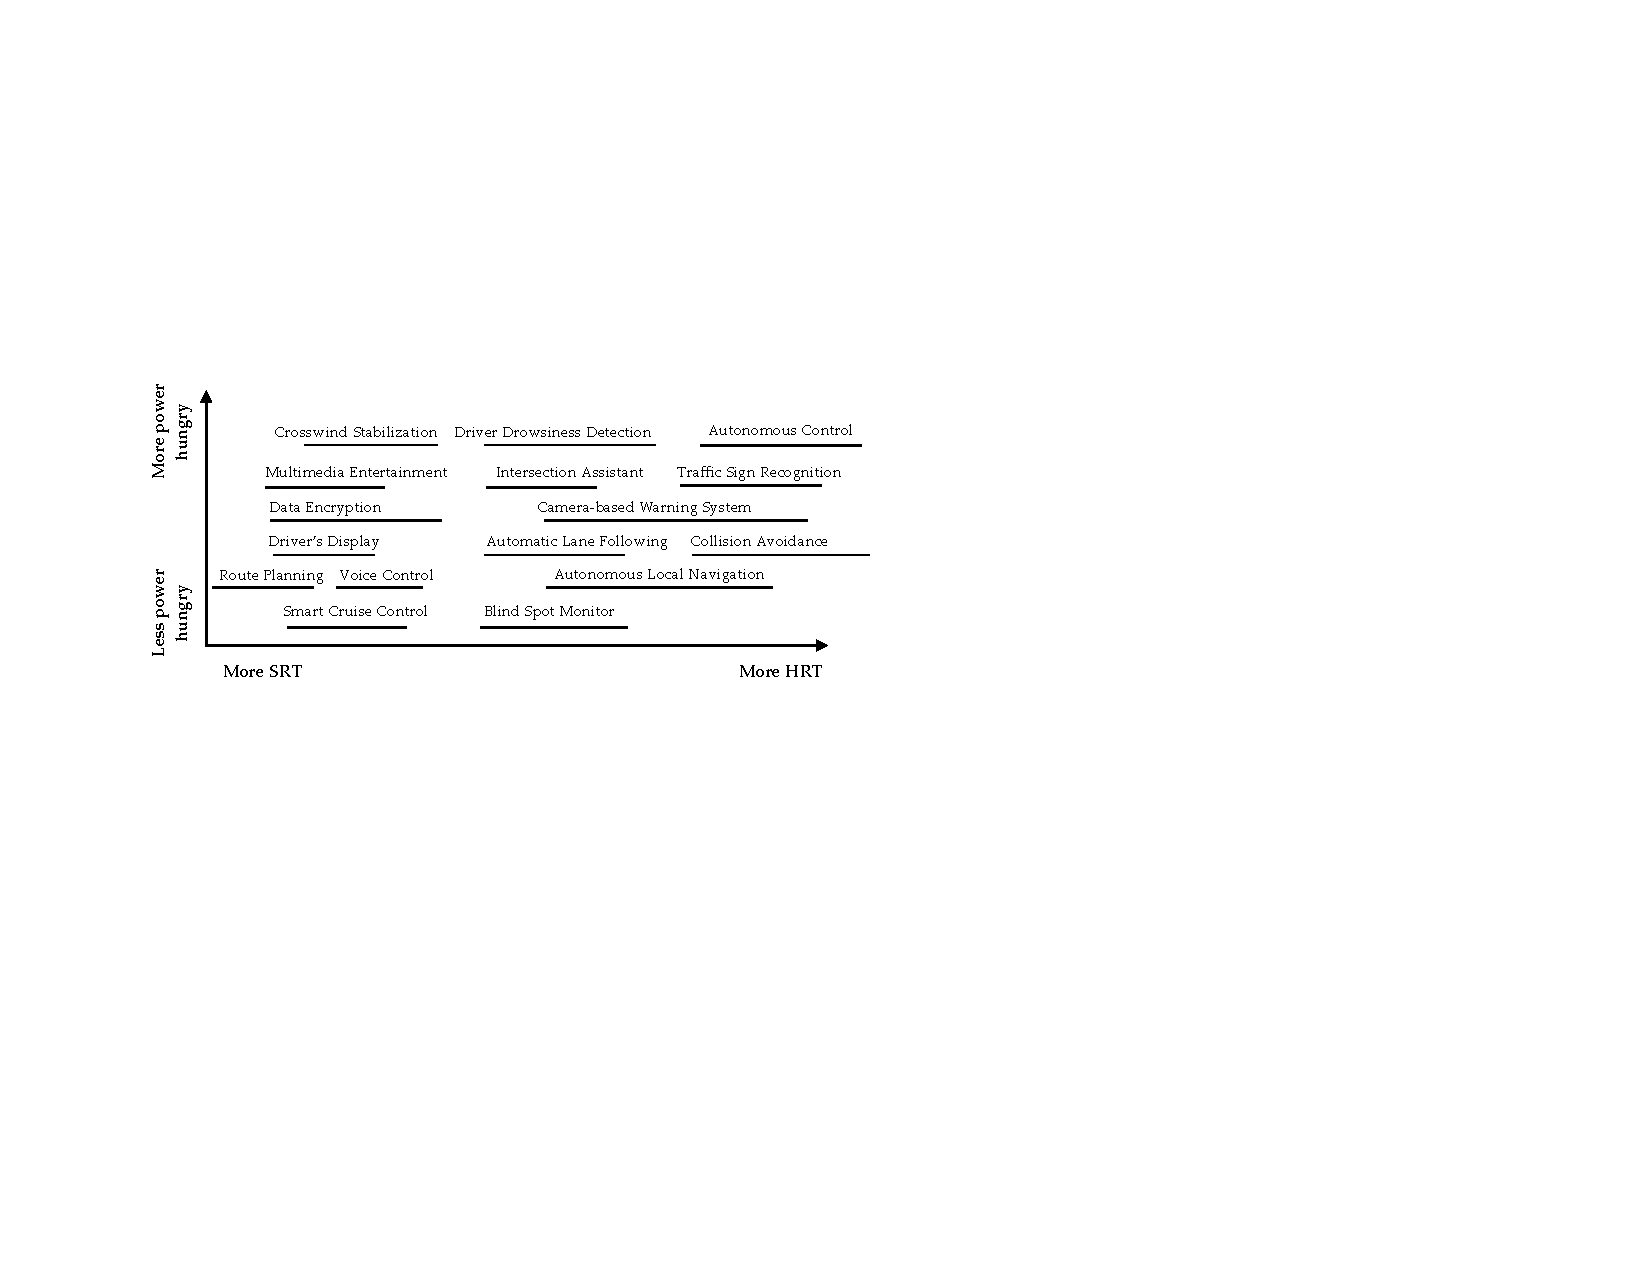
\includegraphics[width=4.6in]{images/automotive.pdf}
\vspace{-2mm}\caption{Spectrum of possible timing and energy requirements for a number of automotive workloads.}
\vspace{-4mm}
\label{fig:automotive}
\end{figure}

\paragraph{Automotive workloads.} 
\label{sec:automotiveworkload}

Heterogeneous computing platforms may be applied in a number of application domains where a wide range of timing and energy constraints are required. A particularly focused application domain we will investigate in this research is advanced driver-assisted automotive systems, where workloads with various timing and energy requirements are seen~\cite{elliott2011real}, as illustrated in Figure~\ref{fig:automotive}.  
The automotive system represents an application domain where using heterogeneous computing platforms to achieve real-time performance and energy efficiency is particularly compelling. 
 In such systems, cores with different performance and energy characteristics can be allocated to workloads with different timing requirements. For example, more powerful cores can be used to process HRT workloads such as traffic sign recognition and collision avoidance; while less powerful but more energy efficient cores can be used to process SRT workloads such as voice control and route planning. Doing so may yield significantly less energy consumption compared to homogeneous platforms. % because less power-hungry workloads do not need to be processed by powerful cores, which results in necessarily high performance at the cost of energy loss.  Due to these reasons, heterogeneous computing platforms such as our targeted ARM's big.LITTLE are expected to see widespread adoption in automotive systems~\cite{armvehicle, armvehicle1, armvehicle2, armvehicle3}. 


\paragraph{Real-time OS.} The OS platform in this project will be an open-source real-time Linux extension called LITMUS$^{\textrm{RT}}$ \cite{LITMUS}. The PI was involved in developing this testbed~\cite{elliott1minimizing, Liudissertation}. The main purpose of LITMUS$^{\textrm{RT}}$ is to provide a useful experimental platform for applied real-time systems research. Currently LITMUS$^{\textrm{RT}}$ extends Linux by implementing a set of common scheduling algorithms as plug-in components. Numerous  publications \cite{elliott1minimizing, elliott1minimizing, Liudissertation, BBBdissertation, clustered, calandrino2008cache, johndissertation} have shown LITMUS$^{\textrm{RT}}$ to be a very valuable testbed for experimentally evaluating real-time scheduling algorithms by considering real system overheads. 
 Since big.LITTLE supports Linux (after setting a scheduler patch to add native big.LITTLE schedulers) and LITMUS$^{\textrm{RT}}$ is developed as a patch to the Linux kernel, we can run LITMUS$^{\textrm{RT}}$ on big.LITTLE for evaluation purposes.